
\chapter{Quantum-limited amplifiers}
\label{c:paramps}

Thus far, I have discussed idealized quantum measurements, and the paradigm of circuit QED in which we can in practice realize coupled quantum systems which implement these measurements.  What I have not yet discussed, however, is how we build the bridge from this quantum world to the classical world in which we interpret our experimental outcomes.  In general, quantum measurements at some point involve one or more stages of \textit{signal amplification}.  This is necessary because the energy and power scales of quantum systems are usually much, much smaller than the energy and power scales of our classical experimental apparatus.  To bridge this gap, we must create some highly sensitive nonlinear coupling between the quantum degree of freedom and a classical degree of freedom.  A classic example of such a coupling is a photomultiplier tube, a device capable of measuring the arrival time and energy of a single optical photon to high precision.  The arrival of a photon creates an ionization event which cascades down a series of metal plates biased with very high voltage, resulting in a very large current pulse.  Considering that the initial photo-ionization event produces a single electron, the total current pulse is equivalent to a signal gain of 70 dB or more \cite{Hakamata2002}.

In the context of superconducting circuits, most all signals are continuous-value microwave fields, usually Gaussian coherent states.  The signal powers are typically quite weak: the resonant frequency and bandwidth of a typical circuit QED cavity are on the other of 5 GHz and 5 MHz, respectively, and the cavity is typically driven with a intracavity field corresponding to a mean cavity occupation $\bar{n}$ on the order of 1 or so.  This corresponds to an output power of $P = \hbar \omega \kappa \bar{n} \sim 1 \times 10^{-16}$ W $ = -130$ dBm.  The typical powers used in analog microwave signal processing in the classical regime at room temperature are on the order of $10^{-3}$ W $= 0$ dBm, so we require about 13 orders of magnitude of amplification to bridge these disparate scales.  However, unlike for destructively detecting the incidence of a single optical photon, we require this amplification to produce a faithfully amplified copy of the continuous-valued input signal while adding as little noise to this signal as possible.  This type of amplification is usually called \textit{linear amplification}, as the output signal $V_{\textrm{out}}(t)$ should obey the relation
\begin{equation}
V_{\textrm{out}}(t) = \sqrt{G} V_{\textrm{in}}(t) + \epsilon(t)
\label{eq:lin_amp}
\end{equation}
where $G$ is the real-valued amplifier power gain, $V_{\textrm{in}}(t)$ is the input signal, and $\epsilon(t)$ is additional uncorrelated noise added by the amplification process.

\section{Amplifier figures of merit}\label{s:amp_figures_of_merit}

\begin{figure*}
\begin{center}
	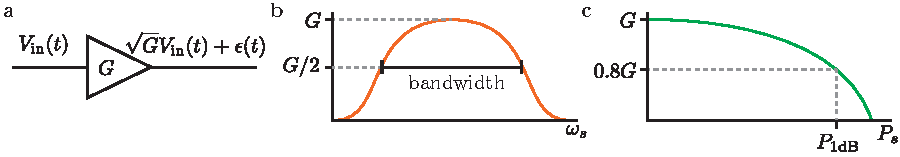
\includegraphics[width = 6in]{paramps_chapter/amp_metrics}
\end{center}
\caption[Amplifier performance metrics]{\textbf{a} A generic amplifier, characterized by its power gain $G$.  The amplifier output contains an amplified copy of the signal as well as some additional noise $\epsilon(t)$.  \textbf{b} The bandwidth of an amplifier is commonly defined as the frequency band over which the amplifier delivers a gain at least as large as $G/2$.  \textbf{c} The input signal power at which the gain is reduced to approximately 80\% (-1 dB) of the small-signal gain is a common figure of merit for amplifier input power handling ability, called the 1 dB input compression power or $P_\textrm{1dB}$.}
\label{fig:amp_metrics}
\end{figure*}

There are several parameters of interest in characterizing the performance of a generic linear amplifier, illustrated in Figure \ref{fig:amp_metrics}.  Ideally, the amplifier faithfully creates an amplified copy of the input signal, increasing the power of that signal by a factor of the power gain $G$.  In the process of amplification, the amplifier also adds some extra noise to the output signal $\epsilon(t)$.  We usually make the approximation that this added noise is independent of the input signal, uncorrelated with itself (white noise), and Gaussian-distributed.  This is a good approximation for thermal noise sources such as Johnson noise and also describes the character of the quantum vacuum noise \cite{clerk_revmod}.

We express this noise in power units over some reference bandwidth $B$, usually taken to be 1 Hz.  We can use Boltzmann's constant $k$  to convert the resulting power into a \textit{noise temperature}
\begin{equation}
T_N = \frac{P_N}{B k}.
\label{eq:Tnoise}
\end{equation}
The output noise temperature of an amplifier is usually \textit{referred} to the input of the amplifier by dividing the output noise temperature by $G$, permitting a straightforward comparison to any relevant noise scales in the input signal.  In general we wish for the input noise of an amplifier to be much smaller than the input signal, permitting a faithful recovery of the input signal from the output.  An extensive discussion of how to measure the noise temperature of a cryogenic amplifier is given in \cite{slichterthesis}.  I will also describe a high-precision technique for making this measurement in chapter \ref{c:twpa_exp}.

The dynamics and amplification mechanism of an amplifier usually provide linear operation only over some finite range of signal frequencies, the \textit{bandwidth} of the amplifier.  Defining bandwidth is somewhat arbitrary, but a commonly-used metric is the frequency band over which the amplifier produces gain at least as large as half of the peak gain, as depicted in Figure \ref{fig:amp_metrics}b.  For gain profiles that are more complex that a simple hump, this definition may not make sense, but it is generally applicable to the amplifiers discussed in this thesis.

Finally, because any amplifier has a finite reservoir of energy to use for amplification, if an input signal becomes too large, the amplifier may not be able to faithfully reproduce it.  This is called \textit{input compression}, and is depicted in Figure \ref{fig:amp_metrics}c.  Generally, when an amplifier becomes compressed, it is no longer able to deliver the full gain $G$ but instead the effective gain starts to decrease as a function of increasing input signal power.  The standard metric for input compression is the input signal power at which the gain of the amplifier is reduced by 1 dB (to approximately $0.8G$), and is the metric discussed in the remainder of this thesis.



\section{Quantum limits on amplification}

Amplification is essentially a form of measurement, as an amplifier is a device that interacts with an input signal and produces an output signal which is correlated with the input signal.  It should be obvious that we wish to minimize the term $\epsilon(t)$ in (\ref{eq:lin_amp}), as this added amplifier noise distorts the output signal and prevents us from recovering the exact input signal.  Considering that quantum mechanics places intrinsic lower bounds on the uncertainty of making various types of measurements, it should come as no surprise that amplification must satisfy some minimum uncertainty relation which constraints just how faithfully the output signal of the amplifier can correlate with the input signal.  The seminal work on deriving a general quantum limit for a linear amplification process was done by Caves in reference \cite{Caves1982a}, though earlier work dates back to 1962 \cite{PhysRev.128.2407,4066904}.  In this section,
 I will follow a more modern review of the subject which I find somewhat more illuminating \cite{clerk_revmod}.

For a continuous, narrowband classical signal $V(t)$ centered at frequency $\omega$, we can write $V(t)$ in terms of a complex number $a$, defining the amplitude and phase of the signal
\begin{equation}
V(t) \propto i ( a e^{-i \omega t} - a^* e^{+i \omega t} ).
\end{equation}
Since we are concerned with the quantum properties of this signal, we must promote $a,a^*$ to the level of quantum ladder operators $a \rightarrow \hat{a}$, $a^* \rightarrow \hat{a}^\dagger$.  For simplicity I'll not bother with the hats for the remainder of the section.  Equivalently, we could instead use the two quadrature amplitude operators I and Q, with functional form
\begin{equation}
\mathrm{I} = \frac{1}{\sqrt{2}} (a^\dagger + a) \quad \mathrm{Q} = \frac{i}{\sqrt{2}} (a^\dagger - a)
\end{equation}
with the commutation relation $[\mathrm{I}, \mathrm{Q}] = i$.  Since the field quadratures are canonically conjugate quantities, we cannot expect to be able to measure both simultaneously to arbitrary precision.

\subsection{Phase-preserving amplification}\label{s:phase_pres_amps}

\begin{figure*}
\begin{center}
	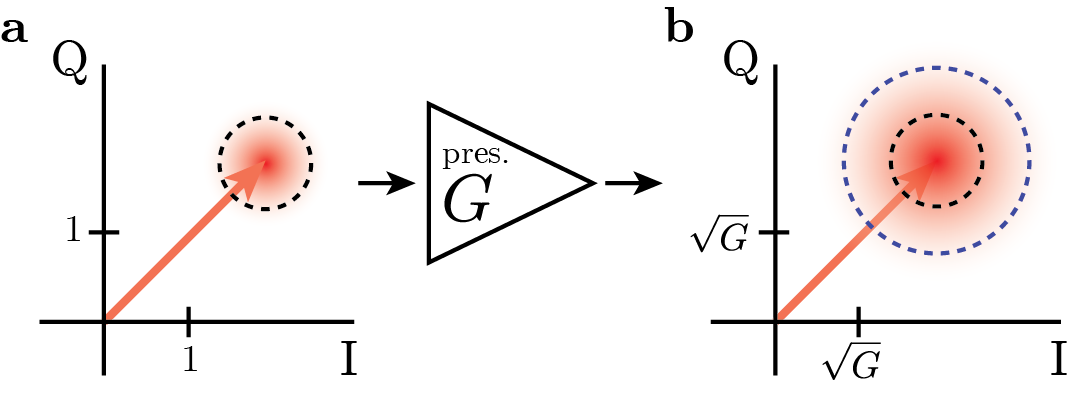
\includegraphics[width = 3.75in]{paramps_chapter/lollipops_pres.png}
\end{center}
\caption[IQ diagram for phase-preserving amplifier]{\textbf{a} IQ diagram of an input coherent state vector, including an uncertainty ``blob'' at the end of the vector representing the vacuum fluctuations.  \textbf{b} The output state, following amplification by a phase-preserving amplifier with gain $G$ (note axis rescaling).  The action of the amplifier has amplified the input vector while maintaining the phase, but has also added some extra noise (dashed purple circle) onto the noise present at the input (black dashed circle).}
\label{fig:lollipops_pres}
\end{figure*}

An amplifier which linearly amplifies both quadratures of the input signal is known as a \textit{phase-preserving} (or \textit{phase-insensitive}) amplifier, as the amplified copy of the signal preserves the phase of the input signal (or, equivalently, the amplification process is insensitive to the phase of the input signal and thus treats both quadratures equally).  A IQ diagram of the action of such an amplifier is shown in Figure \ref{fig:lollipops_pres}.

We consider first the case where an amplifier has just one mode at the input, $a_{\rm in}$, and one at the output, $a_{\rm out}$.  In the usual way, we define the uncertainty in the input field as
\begin{equation}
(\Delta a_{\rm in})^2 \equiv \frac{1}{2} \langle \{a_{\rm in},a_{\rm in}^\dagger \} \rangle - | \langle a_{\rm in} \rangle |^2
\label{eq:gen_uncert}
\end{equation}
with an analogous definition for $(\Delta a_{\rm out})^2$, where the curly brackets $\{~,\}$ indicate anticommutation.  The input and output operators must obey the usual bosonic commutation relations
\begin{equation}
[a_{\rm in},a_{\rm in}^\dagger] = 1, \quad [a_{\rm out},a_{\rm out}^\dagger] = 1.
\label{eq:quad_comm}
\end{equation}
We are seeking a faithful linear relationship between the input and output fields, thus implying that
\begin{equation}
a_{\rm out} = \sqrt{G} a_{\rm in}, \quad a_{\rm out}^\dagger = \sqrt{G} a_{\rm in}^\dagger.
\label{eq:dumb_linear}
\end{equation}
However, it is immediately clear that we cannot simultaneously satisfy (\ref{eq:quad_comm}) and (\ref{eq:dumb_linear}), so the simple linear relationship in (\ref{eq:dumb_linear}) cannot be correct.  We are thus forced to write
\begin{equation}
a_{\rm out} = \sqrt{G} a_{\rm in} + \mathcal{F}, \quad a_{\rm out}^\dagger = \sqrt{G} a_{\rm in}^\dagger + \mathcal{F}^\dagger.
\label{eq:linear_wF}
\end{equation}
What does $\mathcal{F}$ represent, physically speaking?  It cannot be correlated with $a$, else we would violate the commutation relation (\ref{eq:quad_comm}).  Thus we conclude that $\mathcal{F}$ must represent extra noise added by the amplifier.  What is the physical source of this noise?  Since the amplifier provides a power gain $G$, the energy needed to increase the signal power by $G$ must come from \textit{somewhere}, so these extra fluctuations represented by $\mathcal{F}$ are associated with this reservoir of power.

Since $\mathcal{F}$ is uncorrelated with the input signal mode $a_{\rm in}$, $[\mathcal{F},a_{\rm in}] = [\mathcal{F},a_{\rm in}^\dagger] = 0$ and $\langle F a_{\rm in} \rangle = \langle F a_{\rm in}^\dagger \rangle = 0$.  By enforcing the commutation relation (\ref{eq:quad_comm}) for the output field $a_{\rm out}$, we find that
\begin{equation}
[\mathcal{F},\mathcal{F}^\dagger] = 1 - G.
\label{eq:F_comm}
\end{equation}
What does this say about $(\Delta a_{\rm out})^2$, the noise in the output field?  Combining (\ref{eq:gen_uncert}) and (\ref{eq:linear_wF}),
\begin{align}
(\Delta a_{\rm out})^2 &= G (\Delta a_{\rm in})^2 + (1/2) \langle \{ \mathcal{F},\mathcal{F}^\dagger \} \rangle \notag \\
&\geq G(\Delta a_{\rm in})^2 + (1/2) \langle [ \mathcal{F},\mathcal{F}^\dagger ] \rangle  \notag \\
&\geq G(\Delta a_{\rm in})^2 + | G - 1|/2.
\label{eq:output_noise}
\end{align}
In the limit of no gain ($G = 1$), $(\Delta a_{\rm out})^2 = (\Delta a_{\rm in})^2$, and the amplifier need not add any noise.  However, for any gain larger than unity, the output noise must be strictly larger than the amplified input noise.  It is somewhat more illuminating to express this output noise on the same scale as the input noise:
\begin{equation}
(\Delta a_{\rm out})^2 / G \geq (\Delta a_{\rm in})^2 + |1 - 1/G|/2.
\label{eq:output_noise_input_ref}
\end{equation}
It is clear that in the case where $G \gg 1$, the final term will be very small, and so we make the approximation $G \rightarrow \infty$ and find a standard and beautiful result in quantum amplification:
\begin{equation}
(\Delta a_{\rm out})^2 / G \geq (\Delta a_{\rm in})^2 + 1/2.
\label{eq:half_quantum}
\end{equation}
Since we are working in units of photon number, the interpretation of this equation is straightforward.  Much as the ground state of the electromagnetic field intrinsically fluctuates at the level of half a quantum, a general phase-preserving amplifier in the large gain limit must necessarily add fluctuations at the level of half a quantum to the input.

We can go a bit further in understanding this added noise by finding a more detailed form for the extra noise operator $\mathcal{F}$.  From (\ref{eq:F_comm}), we see that for any $G > 1$ the RHS is negative.  If we introduce one additional bosonic mode $d$, corresponding to a mode from which we draw the energy needed for amplification, we can express the extra noise operator as
\begin{equation}
\mathcal{F} = \sqrt{G-1}d^\dagger, \quad \mathcal{F}^\dagger = \sqrt{G-1}d.
\end{equation}
This expression satisfies (\ref{eq:output_noise_input_ref}) as an equality, so an amplifier that realizes this type of operation could potentially add only the minimum half-quantum of noise at high gain.  With this definition for $\mathcal{F}$, we can write the amplifier scattering relation \eqref{eq:linear_wF} as
\begin{equation}
a_{\rm out} = \sqrt{G} a_{\rm in} + \sqrt{G-1} d^\dagger.
\end{equation}

\subsection{Phase-sensitive amplifiers}\label{s:phase_sens_amps}

\begin{figure*}
\begin{center}
	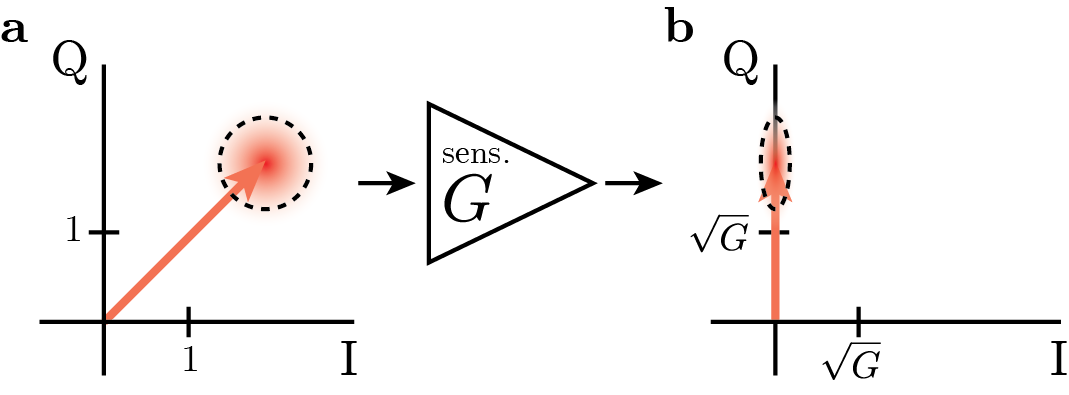
\includegraphics[width = 3.75in]{paramps_chapter/lollipops_sens.png}
\end{center}
\caption[IQ diagram for phase-sensitive amplifier]{\textbf{a} IQ diagram of an input coherent state vector, including an uncertainty ``blob'' at the end of the vector representing the vacuum fluctuations.  \textbf{b} The output state, following amplification by a phase-sensitive amplifier with gain $G$ aligned with the Q quadrature (note axis rescaling).  The action of the amplifier has amplified the input vector along the Q quadrature while de-amplifying the I quadrature.  The resulting ``squeezing'' of the noise is visible in the shape of the noise blob, which has been stretched along Q by $\sqrt{G}$ and compressed along I by $1/\sqrt{G}$; this compression along I implies the translation of the output state vector to the Q axis.}
\label{fig:lollipops_sens}
\end{figure*}

The extra half-quantum of input noise for a phase-preserving amplifier fundamentally arose from our assertion that the amplifier should linearly amplify both quadratures of the signal.  Since these two quadratures do not commute, we could not simultaneously satisfy the commutation relation and the naive requirement of linear amplification.  However, if we relax the linear amplification requirement and limit ourselves to amplifying only one input quadrature, say, the Q quadrature,
\begin{equation}
\mathrm{Q}_{\rm out} = \sqrt{G} \mathrm{Q}_{\rm in}, \quad \mathrm{I}_{\rm out} = \mathrm{I}_{\rm in} / \sqrt{G},
\label{eq:phase_sens}
\end{equation}
then the output fields clearly satisfy the commutation relation.

An amplifier that has an action of this form is known as a \textit{phase-sensitive} (or \textit{phase-nonpreserving}) amplifier, as the amplification process is different depending on the phase of the input signal (or, equivalently, the amplification process does not preserve the input phase of the signal).  Physically speaking, for the action of the amplifier to be different depending on the input phase of the signal implies that the input signal mode and the mode used to supply amplification energy must have a fixed phase relationship.  Here we now speak of $\rm Q$ as the \textit{amplified} quadrature and $\rm I$ as the \textit{deamplified} (or \textit{squeezed}) quadrature.  If the input mode $a$ is a vacuum state, $\rm Q_{out}$ will have fluctuations $\sqrt{G}$ times larger than the vacuum fluctuations, while $\rm I_{out}$ will have fluctuations $\sqrt{G}$ times \textit{smaller} than the vacuum!  This is shown schematically in the IQ plane in Figure \ref{fig:lollipops_sens}.

These are fundamentally quantum states of light, as they require correlations between signal components larger than the limits imposed by classical physics \cite{Loudon1987}.  Because \eqref{eq:phase_sens} satisfies the field quadrature commutation relation, a phase-sensitive amplifier need not intrinsically add any additional noise to the input signal.  In other words, because we are only measuring one half of a pair of non-commuting observables, there is no fundamental limit to how well we can measure that observable, so no added noise term need appear to satisfy such a limit.

\subsection{Quantum efficiency of phase-preserving amplifiers}

The result that a linear phase-preserving amplifier must add an additional half-quantum of noise has led to a great deal of confusion and misunderstanding about the quantum measurement performance of these types of devices.  Since the intrinsic fluctuations of the input mode $a$ correspond to half a quantum, the quantum limit of measuring this mode is often expressed as this same half-quantum.  Thus, if we consider the total input-referred noise of a phase-preserving amplifier to be this half-quantum plus an additional half-quantum, at face value it appears as if a phase-preserving amplifier is forever limited to operating with a quantum efficiency of 0.5.  However, this amounts to a fundamental misunderstanding of the quantum measurement process.

This understanding would be correct if we should place the added half-quantum of noise on the same footing as additional, uncorrelated classical noise in the measurement system.  However, this interpretation is not correct, and can be understood in terms of environmental correlations.  Classical noise $\epsilon(t)$ added by the measurement system is intrinsically part of the incoherent, dissipative classical environment associated with the imperfect measurement apparatus.  If we had perfect control over all of this environment, we could keep track of the exact form of this noise and simply subtract it from the output signal to perfectly recover the underlying signal plus quantum noise.  Thus, any additional classical noise that we do not have an independent record of spoils our perfect quantum-limited measurement.

\begin{figure*}
\begin{center}
	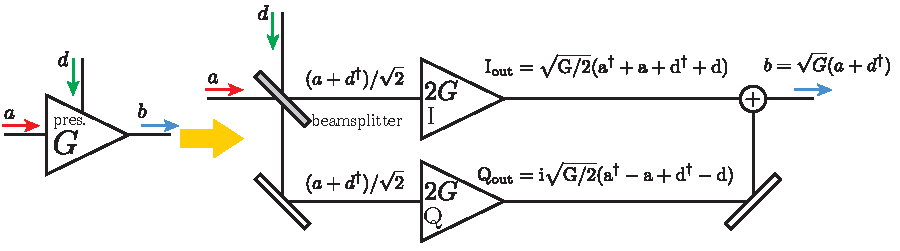
\includegraphics[width = 6in]{paramps_chapter/pres_from_sens}
\end{center}
\caption[Phase-preserving amplifier as two phase-sensitive amplifiers]{A schematic representation of how to create a phase-preserving amplifier with gain $G$ as the combination of two phase-sensitive amplifiers with gain $2G$ and one beam splitter.  We can physically understand the origin of the extra half-quantum of noise in this type of phase-preserving amplifier as the result of adding the second port on the beamsplitter, introducing another vacuum mode $d$.  Note that I have employed the large-gain limit to set $\sqrt{G-1} = \sqrt{G}$ and eliminate the squeezed quadratures from the outputs of the phase-sensitive amplifiers.}
\label{fig:pres_from_sens}
\end{figure*}

The extra minimum noise fundamentally associated with the extra mode needed in a phase-preserving amplifier, however, is not of this form.  Ideally, there is no record of these fluctuations imprinted in an environment beyond our control, so this noise is \textit{fundamentally indistinguishable} from the intrinsic quantum noise of the input mode.  Thus, these added fluctuations do not spoil the efficiency of our measurement.  We can loosely define the measurement efficiency $\eta$ as
\begin{equation}
\eta = \frac{\textrm{the information we collect}}{\textrm{the information we collect } + \textrm{ the information we lost}}.
\label{eq:eta_heur}
\end{equation}
Since the added quantum fluctuations in the extra mode are not correlated with any unmeasured degrees of freedom, we have not lost any information, and a perfect phase-preserving amplifier still has a quantum efficiency of unity once the quantum limit is correctly defined.

This idea can be made more clear by introducing a simple model for a phase-preserving amplifier by combining two phase-sensitive amplifiers, as shown in Figure \ref{fig:pres_from_sens}.  It is clear in this setup that at no point do we lose any information from the mode $a$, nor do we introduce any extra uncorrelated classical noise.  The only difference is the introduction of a beam splitter, adding an extra vacuum port through which the mode $d$ enters the system.  One way to understand the effect of the extra input vacuum mode is that the additional half-quantum of noise does not decrease the efficiency of the measurement, but merely reduces the \textit{strength} of that measurement by a factor of two.  Note that we have had to employ phase-sensitive amplifiers with gain $2G$ to model a phase-preserving amplifier of gain $G$.  This implies that regardless of which type of amplifier we use, we will still achieve quantum-limited measurement back-action as described in section \ref{s:cQED_backaction}.

\section{Practical ultra-low-noise microwave-frequency amplifiers}

Realizing microwave-frequency amplifiers that saturate these lower bounds on added noise is a very nontrivial task.  The input signals are very weak, and, moreover, the energy corresponding to the vacuum fluctuations at the input of the amplifier is extremely small.  We can use Boltzmann's constant to convert the characteristic energy scale of the vacuum fluctuations to a noise temperature $T = \hbar \omega / 2 k = 144$ mK at 6 GHz.  For the fields to be in their ground state, the thermal temperature of the environment must be about an order of magnitude lower than this still, implying an amplifier capable of operating at temperatures of a few tens of millikelvin.

The general design approach for building low-noise microwave amplifiers for operation at cryogenic temperatures utilizes high-quality microwave-frequency semiconductor transistors \cite{Wadefalk2003} made from high-electron-mobility transistors (HEMTs).  HEMT amplifiers are capable of operation at temperatures as low as a few kelvin, and the best devices achieve input-referred noise temperatures as low as 2 or 3 K.  This is still about an order of magnitude larger than the quantum limit!  We therefore need a different type of amplifier entirely, capable of operating at temperatures much lower than the quantum noise temperature.  We will still need HEMT amplifiers in our measurements, as they provide an intermediate stage of amplification to build the bridge to room temperature, providing about 40 dB of gain over a large bandwidth (as large as 10 GHz or more) with a very high input compression power (on the order of 0.1 mW).

In the same way that we turned to superconductors in Chapter \ref{c:scqb} to realize electrical circuits that behaved as coherent quantum systems, we likewise turn to superconductors once again to realize nearly ideal quantum amplifiers.  To build an amplifier, we require an element in our system which behaves in a nonlinear fashion, permitting the modulation created by a small input signal to produce a very large change in the system, realizing gain.  Furthermore, if we wish to couple two modes of the electromagnetic field, we require some term in the wave equation that mixes these different modes, which a purely linear wave equation does not achieve.  In the same way that we utilized Josephson junctions to make harmonic LC oscillators into anharmonic oscillators that behaved more like atoms, we will employ the Josephson nonlinearity once again, this time to create circuits that efficiently couple different electromagnetic modes.

\subsection{Parametric amplifiers}

The operating principle for the lowest-noise superconducting amplifiers is the paradigm of \textit{parametric amplification}.  The idea is that rather than directly adding energy to the signal mode, a source of energy is instead used to modulate a parameter of a dynamical system, producing amplification of a signal mode incident on the system.  A classic example of this process is a playground swingset.  The motion of a person swinging on the swing can be driven by walking up and pushing them at the right moment, directly adding energy into the swing's motion.  Alternatively, the person on the swing can modulate the moment of rotational inertia of the entire swing by slightly increasing and decreasing the length of the swing at the right moments, ``pumping'' the swing, and thus adding energy to the swing's motion and amplifying the initial conditions.

In a general parametric process, we supply energy from a pump wave ($\omega_p$) which couples to at least two other modes, traditionally called the signal ($\omega_s$) and the idler ($\omega_i$).  The relationship between these quantities is essentially a statement of energy conservation, and comes in two minimal flavors: \textit{three-wave mixing}, where one pump photon is converted to one signal and one idler photon as
\begin{equation}
\omega_p = \omega_s + \omega_i;
\label{eq:3wave}
\end{equation}
and \textit{four-wave mixing}, where two pump photons are converted to one signal and one idler photon as
\begin{equation}
\omega_p + \omega_p = \omega_s + \omega_i.
\label{eq:4wave}
\end{equation}
If the signal and idler modes are the same ($\omega_s = \omega_i$), the process is called a \textit{degenerate} process, and $\omega_p$ will be an integer multiple of $\omega_s$.  This type of degenerate process implies a well-defined phase relationship between the pump and signal modes and thus realizes a phase-sensitive process.  I will focus on four-wave mixing processes, as none of the devices described in this thesis operate in a three-wave mixing mode\footnote{Parametric amplifiers based on the Josephson Parametric Converter are an example of a three-wave mixing device \cite{JPCNature}.}.

\subsection{Lumped-element Josephson parametric amplifiers}

The Josephson junction provides a convenient nonlinear circuit element with which to realize a parametric process.  When the junction is driven with a strong pump wave $\omega_p$, the Josephson inductance is modulated by the current in this wave roughly as $I_p(t)^2$; since this quantity is always positive, the inductance is effectively modulated at $2 \omega_p$.  To utilize this nonlinear modulation as an amplifier, the junction is embedded in an LC resonator; in fact, the circuit diagram for a simple lumped-element Josephson parametric amplifier (LJPA) is identical to that for a transmon qubit \cite{PhysRevA.86.013814} but with a much weaker anharmonicity, resulting in a classical nonlinear oscillator.

\begin{figure*}
\begin{center}
	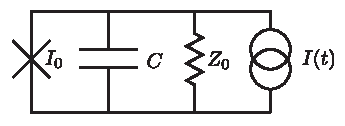
\includegraphics[width = 2.3in]{paramps_chapter/JPA_circuit}
\end{center}
\caption[Circuit model for LJPA]{Circuit model for a Josephson nonlinear resonator operated as a LJPA.  The nonlinear resonator is formed from the junction and capacitor at left, loaded by a transmission line modeled as a lumped impedance $Z_0$ and driven by an ideal current source $I(t)$.}
\label{fig:JPA_circuit}
\end{figure*}

The precise physics behind the operation of the LJPA is beyond the scope of relevance for this thesis, and has already been treated extensively in other works.  The general method to solve for the behavior of the LJPA is to start from the circuit model shown in Figure \ref{fig:JPA_circuit}.  Applying Kirchoff's laws permits the derivation of a differential equation for the junction phase difference $\delta(t)$, which will involve a nonlinear term proportional to $\sin[{\delta}(t)]$ due to the Josephson current-phase relation (\ref{eq:CPR}).  Approximating this term to the lowest nonlinear order of $\delta(t)^3$ results in the equation of motion of a classical Duffing oscillator, which can be explicitly solved for $\delta(t)$ in the presence of a strong drive.  This approach is described in detail in references \cite{slichterthesis,castaellanosthesis}.  Another approach, interesting for explicitly treating the quantum noise performance of the device, begins from the Hamiltonian for a first-order nonlinear harmonic oscillator, and is extensively described in reference \cite{eichlerthesis}.

\subsection{Performance and limitations of LJPAs}\label{s:jpa_perf}

We can consider a LJPA as a black box amplifier and characterize it using the figures of merit described in section \ref{s:amp_figures_of_merit}.  JPAs are generally operated with a gain of about 20 dB, sufficiently high to ensure that amplified input quantum fluctuations are much larger than the noise added by the following HEMT amplifier.  The input-referred noise temperatures can be close to the quantum limit, often within a factor of 2.  The main limitations for LJPAs are bandwidth and input power saturation, both of which are fundamentally related to the use of a nonlinear resonator as the geometry of the amplifier.

The need for a resonant geometry is essentially to enhance the coupling between the signal wave and the modulation of the Josephson junction.  The small-signal resonant frequency of this circuit is given by
\begin{equation}
\omega_0 = \frac{1}{\sqrt{L_JC}} = \sqrt{\frac{2\pi I_0}{\Phi_0 C}}.
\label{eq:w0_RLC}
\end{equation}
The bandwidth $B$ in the small-signal regime is related to the inverse of the quality factor, given simply by the standard equation for a LC oscillator damped by the coupling to a feedline of real impedance $Z_0$
\begin{equation}
Q = \omega_0 Z_0 C
\label{eq:Q_RLC}
\end{equation}
where $B \sim \omega_0/Q$.  This is a good approximation for large values of $Q$, but not entirely correct for small $Q$.  As the resonator is driven near resonance by a strong pump, the parametric process leads to gain as well as a reduction in bandwidth.  This tradeoff is known as the \textit{gain-bandwidth product}, and is roughly expressed as
\begin{equation}
B\sqrt{G} \propto \frac{1}{Q}.
\label{eq:g_bw_prod}
\end{equation}

Typical gain-bandwidth products for LJPAs are on the order of 100 MHz, implying $B = 10$ MHz with 20 dB gain \cite{Castellanos-Beltran2007,JPCNature,Hatridge:2011zr}.  Some devices have been demonstrated with gain-bandwidth products on the order of 1 GHz 
\cite{Mutus2014}.

The input compression power is determined by the amount of pump power available for amplification.  Roughly speaking, for the amplifier to remain linear, the fraction of the energy in the pump transferred to the signal should be very small, on the order of 1\% or -20 dB.  For an amplifier with 20 dB gain, this implies that the 1 dB compression power will be about 40 dB smaller than the pump power.  The maximum pump power than can be utilized is limited by the nonlinear dynamics of the resonator and is typically constrained to be 5-10\% of the critical current \cite{slichterthesis}.  For typical parameters, the 1 dB compression power is about -130 dBm \cite{Hatridge:2011zr}, though improved devices have enhanced this by as much as 20 dB \cite{Eichler2014a,Mutus2014}.

The gain-bandwidth product is the most challenging design constraint in improving the performance of LJPAs.  To increase both the gain of the amplifier and the bandwidth simultaneously, we can decrease $Q$.  We cannot make $Q$ arbitrarily small, however, as eventually higher-order nonlinear processes become important and prevent stable amplifier operation.  An approximate requirement for stability is
\begin{equation}
Q p \gtrsim 5
\label{eq:Q_p_prod}
\end{equation}
where $p = L_J / L_{tot}$ is the participation ratio of the Josephson inductance to the total inductance \cite{Weber2014a}.  In general there will always be some stray inductance which constrains $p < 1$.

We typically wish to keep the center frequency $\omega_0$ of the amplifier fixed at some specific value, requiring that we maintain a fixed ratio $I_0 / C$.  Thus, if we decrease $Q$ by making $C$ smaller, we must also reduce the junction critical current, thus reducing the input compression power.  One possible way to avoid this problem is by decreasing the environmental loading impedance $Z_0$ instead of $C$ by utilizing an impedance transformer to convert the standard 50 $\Omega$ environment to a lower value.  One device has been demonstrated with $Z_0 = 15$ $\Omega$ and realized a remarkably large bandwidth, though much of this improvement was related to a coincidental frequency dependence in $Z_0$ formed by the long propagation length of the impedance transformer rather than the reduction in $Z_0$ itself \cite{Mutus2014}.

One final constraint intrinsic to LJPA operation is the necessity of a separate non-reciprocal circuit element.  A resonator-based amplifier is intrinsically a 1-port device; this can be intuitively understood by the simultaneous need to efficiently couple the input signal to the resonator and efficiently couple the amplified field back out.  For a simple geometry, due to the reciprocal nature of the circuit topology, any port into the device that functions as an input will function just as effectively as an output.  Thus, the amplified output field leaves the amplifier through the same port through which it entered.  We must then use a non-reciprocal element to separate the outgoing signal mode from the incoming mode.  Microwave circulators are usually employed for this purpose, and do the job quite effectively.  However, these components are large, magnetic, expensive, and lossy.  Josephson-based parametric amplifiers with intrinsic directionality have been realized using a much more exotic circuit topology \cite{Abdo2014}, though the bandwidth and dynamic range of these devices are quite limited.

\section{Traveling-wave amplifiers}

For several applications of interest, the design constraints inherent in the LJPA are simply too stringent to realize an amplifier that simultaneously achieves large gain, large bandwidth, and large dynamic range.  For example, one common approach utilizing one amplifier and one transmission line to readout several qubits simultaneously is frequency-division multiplexing, which requires a bandwidth on the order of 50 MHz per qubit and power handling corresponding to about -110 dBm per qubit \cite{Barends2014,Riste2014}.  Furthermore, there are applications such as fault-tolerant quantum computing where the need for a circulator is a major impediment to scaling up the measurement system to thousands of qubits.  These constraints are inherent to the resonant geometry of the amplifier, so a natural question arises: is it possible to realize a Josephson amplifier that does not intrinsically utilize a resonant mode?

The inspiration for such a device comes from the optical domain.  Optical fibers have a weak, intrinsic nonlinearity which is exploited to make amplifiers \cite{Hansryd:2015uq}.  The general idea, then, is to exchange the enhanced coupling between the incident modes and the nonlinear element provided by the resonator for a very long co-propagation length through an extended nonlinear medium.  Because the pump and signal waves are now propagating in a single spatial direction, the gain provided by the amplifier is intrinsically directional and thus naturally operates as a 2-port device, eliminating the need for a external non-reciprocal element to separate the input and output modes.  The propagation length required in these optical fiber parametric amplifiers (OFPAs) is on the order of 100 m or more, owing to the very weak nonlinearities intrinsic to nonlinear optical systems.

In addition to the energy conservation criteria described previously (\ref{eq:4wave}), the traveling waves now also carry nonzero momentum, ascribed to the dispersion relation intrinsic to the waveguide in which the waves propagate.  For efficient mixing to occur, the process must conserve momentum; for four-wave mixing, we require
\begin{equation}
2 k_p = k_s + k_i
\label{eq:4wave_phase}
\end{equation}
where $k_x$ is the wavevector for mode $x \in \{p,s,i\}$.  This condition combined with (\ref{eq:4wave}) amounts to a constraint on the shape of the dispersion relation $k(\omega)$.  Since the spatial phase evolution of the modes is proportional to $k$, this momentum-matching constraint is generally called \textit{phase matching} in the literature of nonlinear optics.  Achieving phase matching is a central problem in nonlinear optical systems, and is likewise crucial to the efficient functioning of traveling-wave amplifiers.  I will leave a detailed discussion of this problem and its solution for chapter \ref{c:twpa_theory}.

\subsection{Josephson traveling-wave amplifiers}

Creating a superconducting amplifier analogous to a OFPA is not a new idea; a theoretical proposal for this type of device was made in 1985 \cite{Sweeny1985}, and an experimental realization of the device was created at Bell Labs in 1996 by Yurke \textit{et al} \cite{Yurke:1996ys}.  These works entirely ignored the issue of phase matching; furthermore, the Yurke device was created by loading the center trace of a co-planar waveguide (CPW) structure with 1000 Josephson junctions, producing a nonlinear transmission line with an impedance of 430 $\Omega$.  Because of this poor matching to the environment, the device was operated with one end shorted as a reflection amplifier and did not produce a compelling demonstration of traveling-wave performance.  The bandwidth of the amplifier was also quite small, only 125 MHz at a gain of 12 dB, comparable to a standard LJPA.

\begin{figure*}
\begin{center}
	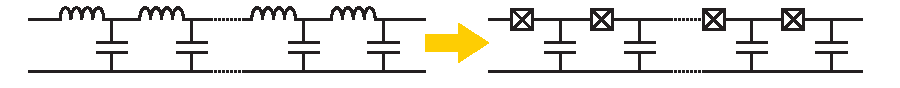
\includegraphics[width = 6in]{paramps_chapter/TWPA_circuit}
\end{center}
\caption[Circuit model for simple Josephson traveling-wave amplifier]{``LC ladder" lumped-element transmission line, and equivalent nonlinear lumped-element transmission line utilizing the Josephson inductance.}
\label{fig:TWPA_circuit}
\end{figure*}

\begin{figure*}
\begin{center}
	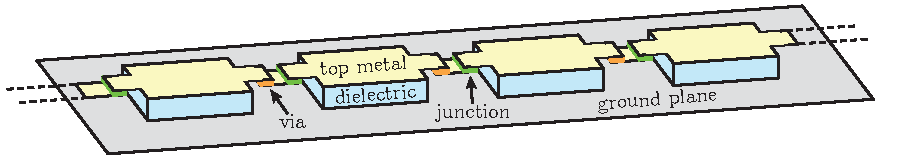
\includegraphics[width = 6in]{paramps_chapter/TWPA_geometry}
\end{center}
\caption[JTWPA in quasi-microstrip geometry]{A quasi-microstrip geometry to realize a low-impedance JTWPA.  The overall geometry looks something like a microstrip, with a center conductor (light yellow) situated on top of a ground plane (gray) with an intermediate dielectric layer (light blue).  Here, the center conductor is periodically interrupted by a Josephson junction (green).  A inter-layer via (orange) is used to make electrical contact with the bottom of the junction trilayer.}
\label{fig:TWPA_geometry}
\end{figure*}

Early attempts to produce a Josephson traveling-wave parametric amplifier (JTWPA) at QNL were performed by Ofer Naaman and Dan Slichter following the existing literature on the subject.  At this point in time the phase matching issue was not well understood, so early device designs looked much like straightforward nonlinear lumped-element transmission lines with Josephson junctions providing the inductance, as shown in Figure \ref{fig:TWPA_circuit}.  The main innovation at this point in time was the introduction of a new physical geometry for the transmission line; rather than utilizing a CPW structure as in the Bell Labs device, we created a kind of quasi-microstrip geometry shown in Figure \ref{fig:TWPA_geometry}.  By employing a parallel-plate capacitor geometry, the capacitance to ground per junction can be made much larger than in a CPW, allowing for the transmission line to be well matched to 50 $\Omega$.

Due to fabrication difficulties, these early devices never delivered breathtaking amplifier performance and were plagued by large, unknown losses; parametric gain was observed, however, encouraging continued development.  These results are described in Slichter's thesis \cite{slichterthesis}.  To understand what might be limiting this performance, we embarked on a major theoretical effort to understand the JTWPA, finally culminating in the practical device described in this thesis.  The full theory of the JTWPA and extensive experimental results are the subject of chapters \ref{c:twpa_theory} and \ref{c:twpa_exp}, respectively.





















